%% BioMed_Central_Tex_Template_v1.05
%%                                      %
%  bmc_article.tex            ver: 1.05 %
%                                       %


%%%%%%%%%%%%%%%%%%%%%%%%%%%%%%%%%%%%%%%%%
%%                                     %%
%%  LaTeX template for BioMed Central  %%
%%     journal article submissions     %%
%%                                     %%
%%         <27 January 2006>           %%
%%                                     %%
%%                                     %%
%% Uses:                               %%
%% cite.sty, url.sty, bmc_article.cls  %%
%% ifthen.sty. multicol.sty		       %%
%%									   %%
%%                                     %%
%%%%%%%%%%%%%%%%%%%%%%%%%%%%%%%%%%%%%%%%%


%%%%%%%%%%%%%%%%%%%%%%%%%%%%%%%%%%%%%%%%%%%%%%%%%%%%%%%%%%%%%%%%%%%%%
%%                                                                 %%	
%% For instructions on how to fill out this Tex template           %%
%% document please refer to Readme.pdf and the instructions for    %%
%% authors page on the biomed central website                      %%
%% http://www.biomedcentral.com/info/authors/                      %%
%%                                                                 %%
%% Please do not use \input{...} to include other tex files.       %%
%% Submit your LaTeX manuscript as one .tex document.              %%
%%                                                                 %%
%% All additional figures and files should be attached             %%
%% separately and not embedded in the \TeX\ document itself.       %%
%%                                                                 %%
%% BioMed Central currently use the MikTex distribution of         %%
%% TeX for Windows) of TeX and LaTeX.  This is available from      %%
%% http://www.miktex.org                                           %%
%%                                                                 %%
%%%%%%%%%%%%%%%%%%%%%%%%%%%%%%%%%%%%%%%%%%%%%%%%%%%%%%%%%%%%%%%%%%%%%


\NeedsTeXFormat{LaTeX2e}[1995/12/01]
\documentclass[10pt]{bmc_article}    



% Load packages
\usepackage{cite} % Make references as [1-4], not [1,2,3,4]
\usepackage{url}  % Formatting web addresses  
\usepackage{ifthen}  % Conditional 
\usepackage{multicol}   %Columns
\usepackage[utf8]{inputenc} %unicode support
%\usepackage[applemac]{inputenc} %applemac support if unicode package fails
%\usepackage[latin1]{inputenc} %UNIX support if unicode package fails
\urlstyle{rm}
 
 
%%%%%%%%%%%%%%%%%%%%%%%%%%%%%%%%%%%%%%%%%%%%%%%%%	
%%                                             %%
%%  If you wish to display your graphics for   %%
%%  your own use using includegraphic or       %%
%%  includegraphics, then comment out the      %%
%%  following two lines of code.               %%   
%%  NB: These line *must* be included when     %%
%%  submitting to BMC.                         %% 
%%  All figure files must be submitted as      %%
%%  separate graphics through the BMC          %%
%%  submission process, not included in the    %% 
%%  submitted article.                         %% 
%%                                             %%
%%%%%%%%%%%%%%%%%%%%%%%%%%%%%%%%%%%%%%%%%%%%%%%%%                     


%%\def\includegraphic{}
%%\def\includegraphics{}



\setlength{\topmargin}{0.0cm}
\setlength{\textheight}{21.5cm}
\setlength{\oddsidemargin}{0cm} 
\setlength{\textwidth}{16.5cm}
\setlength{\columnsep}{0.6cm}

\newboolean{publ}

%%%%%%%%%%%%%%%%%%%%%%%%%%%%%%%%%%%%%%%%%%%%%%%%%%
%%                                              %%
%% You may change the following style settings  %%
%% Should you wish to format your article       %%
%% in a publication style for printing out and  %%
%% sharing with colleagues, but ensure that     %%
%% before submitting to BMC that the style is   %%
%% returned to the Review style setting.        %%
%%                                              %%
%%%%%%%%%%%%%%%%%%%%%%%%%%%%%%%%%%%%%%%%%%%%%%%%%%
 

%Review style settings
\newenvironment{bmcformat}{\begin{raggedright}\baselineskip20pt\sloppy\setboolean{publ}{false}}{\end{raggedright}\baselineskip20pt\sloppy}

%Publication style settings
%\newenvironment{bmcformat}{\fussy\setboolean{publ}{true}}{\fussy}



% Begin ...
\begin{document}
\begin{bmcformat}


%%%%%%%%%%%%%%%%%%%%%%%%%%%%%%%%%%%%%%%%%%%%%%
%%                                          %%
%% Enter the title of your article here     %%
%%                                          %%
%%%%%%%%%%%%%%%%%%%%%%%%%%%%%%%%%%%%%%%%%%%%%%

\title{Xander: Gene Targeted Metagenomics}
 
%%%%%%%%%%%%%%%%%%%%%%%%%%%%%%%%%%%%%%%%%%%%%%
%%                                          %%
%% Enter the authors here                   %%
%%                                          %%
%% Ensure \and is entered between all but   %%
%% the last two authors. This will be       %%
%% replaced by a comma in the final article %%
%%                                          %%
%% Ensure there are no trailing spaces at   %% 
%% the ends of the lines                    %%     	
%%                                          %%
%%%%%%%%%%%%%%%%%%%%%%%%%%%%%%%%%%%%%%%%%%%%%%


\author{Jordan A Fish\correspondingauthor$^{1,2}$%
       \email{Jordan Fish\correspondingauthor - fishjord@msu.edu}%
      \and
         Yanni Sun$^2$%
         \email{Yanni Sun - yannisun@msu.edu}
       \and 
         James M Tiedje$^1$%
         \email{James M Tiedje - tiedjej@msu.edu}%
       \and 
         James R Cole$^1$%
         \email{James R Cole - colej@msu.edu}%
      }
      

%%%%%%%%%%%%%%%%%%%%%%%%%%%%%%%%%%%%%%%%%%%%%%
%%                                          %%
%% Enter the authors' addresses here        %%
%%                                          %%
%%%%%%%%%%%%%%%%%%%%%%%%%%%%%%%%%%%%%%%%%%%%%%

\address{%
    \iid(1)Center for Microbial Ecology, Michigan State University
    \iid(2)Department of Computer Science and Engineer, Michigan State University
}%

\maketitle

%%%%%%%%%%%%%%%%%%%%%%%%%%%%%%%%%%%%%%%%%%%%%%
%%                                          %%
%% The Abstract begins here                 %%
%%                                          %%
%% The Section headings here are those for  %%
%% a Research article submitted to a        %%
%% BMC-Series journal.                      %%  
%%                                          %%
%% If your article is not of this type,     %%
%% then refer to the Instructions for       %%
%% authors on http://www.biomedcentral.com  %%
%% and change the section headings          %%
%% accordingly.                             %%   
%%                                          %%
%%%%%%%%%%%%%%%%%%%%%%%%%%%%%%%%%%%%%%%%%%%%%%


\begin{abstract}
        % Do not use inserted blank lines (ie \\) until main body of text.
        \paragraph*{Background:} Metagenomics can provide important insight in to microbial communities.  It can be used to analyze entire genomes and takes full advantage of increasing sequencing capacity. However analyzing large metagenomic datasets has proven to be very computationally challenging with even modest metagenomic datasets requiring 256 gigabytes of memory or more (cite hmp assembly, titus). As dataset size progresses from 50 gigabases to 500 gigabases and beyond new methods are needed for deriving understanding from metagenomic datasets.  We present a method for assembling protein coding sequences for gene(s) of interest from a metagenomic dataset which uses a compressible graph format and only assembles targeted data to drastically reduce the amount of memory and processing time required.
      
        \paragraph*{Results:} \ldots

        \paragraph*{Conclusions:} \ldots
\end{abstract}



\ifthenelse{\boolean{publ}}{\begin{multicols}{2}}{}




%%%%%%%%%%%%%%%%%%%%%%%%%%%%%%%%%%%%%%%%%%%%%%
%%                                          %%
%% The Main Body begins here                %%
%%                                          %%
%% The Section headings here are those for  %%
%% a Research article submitted to a        %%
%% BMC-Series journal.                      %%  
%%                                          %%
%% If your article is not of this type,     %%
%% then refer to the instructions for       %%
%% authors on:                              %%
%% http://www.biomedcentral.com/info/authors%%
%% and change the section headings          %%
%% accordingly.                             %% 
%%                                          %%
%% See the Results and Discussion section   %%
%% for details on how to create sub-sections%%
%%                                          %%
%% use \cite{...} to cite references        %%
%%  \cite{koon} and                         %%
%%  \cite{oreg,khar,zvai,xjon,schn,pond}    %%
%%  \nocite{smith,marg,hunn,advi,koha,mouse}%%
%%                                          %%
%%%%%%%%%%%%%%%%%%%%%%%%%%%%%%%%%%%%%%%%%%%%%%




%%%%%%%%%%%%%%%%
%% Background %%
%%
\section*{Background}Metagenomics has the potential to help answer many questions but has faced scalability challenges stemming from the amount of raw sequencing data required for metagenomic analysis.  Metagenomic assembly has been an area of interest in recent years with the early datasets assembled using single genome assembly approaches.  The tendency for single genome assemblers to only assemble a few dominant organisms has been an impetus to develop metagnomic specific assembly methods.  Currently metagenomic assembly approaches focus on separating individual organism genomes out of the metagenomic data to be worked on individual (Metavelvet, Partitioning).  

We propose a gene targeted approach for assembling metagenomic datasets: HMMgs.  HMMgs is a De Bruijn Graph (cite) assembler but unlike traditional approaches that find either a Eulerian or Hamiltonian path through the graph, we use a protein profile Hidden Markov Model (HMM) (cite) to target specific paths in the graph and guide assembly. By using an HMM we can explore most probable paths first to limit the amount of the graph we must explore along with obtaining a measure of how well the resulting assembled sequence is from the supplied model.  Using this gene targeted approach allows for a functional based analysis of the data,by allowing us to directly examine genes involved in biologically interesting pathways.

Gene targeted assembly is less resource intensive and faster than whole genome assembly.  In addition to the De Bruijn Graph, only small paths relative to the graph's size must be kept in memory.  Further reduction in the memory usage are achieved by using a probabilistic data structure for holding the De Bruijn Graph in memory, a Bloom filter \cite{Bloom1970} (cite kmer percolation).  By targeting relatively small segments of the metagenome by using an HMM to guide assembly, we limit how much of the graph must be explored during assembly, providing a speed up over whole genome approaches.

Our Method is more sensitive than whole genome assembly and more specific than individual read-based approaches fro functional analysis.  By using an assembly approach we have more context from which to make a determination as to whether a stretch of sequence belongs to the target gene or not, increasing our sensitivity compared to read based approaches.  Using HMM probabilities to guide local assembly helps to ensure we explore the most relevant paths to assemble sequences most likely to represent the gene of interest, increasing our sensitivity compared to uniform global assembly.

We use a graph search based approach to assemble the targeted genes.  We create a graph structure on demand that is a combination of a De Bruijn Graph and HMM.  A De Bruijn Graph is a graph where vertices represent fixed K-length words (K-mers) and edges link vertices that share K-1 word.  A HMM can also be thought of as a graph in which each vertex represents a model state and edges represent allowed transitions between states.  By combining the two we create a graph structure that can be easily searched using existing graph search algorithms.

 
%%%%%%%%%%%%%%%%%%%%%%%%%%%%
%% Results and Discussion %%
%%
\section*{Results and Discussion}
We tested HMMgs on three approx. 50 gigabase Illumina GAII soil metagenomes: two Great Prairie Challenge Iowa datasets, Iowa Corn and Iowa Prairie, and one Miscanthus Rizosphere set from a GLBRC plot at the Kellog Biological Station. We focused on Nitrogen Reductase (nifH) and 50S ribosomal protein L2 rplB for these datasets.  NifH is important in nitrogen fixation and expected to be found in the datasets albiet at low levels. The rplB gene coding for ribosomal protein L2 is present in all bacteria and archaea and was used to benchmark our program on highly abundant genes.

\subsection*{Preparing Genes of Interest}
For each gene of interest we selected a set high-quality seed sequences to build a HMM model and a larger set used to identify possible starting Kmers.  Seed sequences were obtained from the Ribosomal Database Project's Functional Gene Repository (FGR) (cite) [How were these selected?].  Sequences for the larger reference set were also downloaded from the FGR.  All sequences that covered at least 90\% of the HMM and with a good bits saved score, dependent on the gene, were selected as the larger reference set.

We used the seed sequences to build an HMM for each gene using a modified version of HMMER3 (cite). While testing HMMgs we found that HMMER3's default delete and insert prior probabilities appeared much higher than seen in the genes we were examining an such high priors sometimes caused extensive searching of nonproductive insert and delete paths. with our metagenomic data. We modified HMMER3's source code to change the prior probabilities for the $delete \rightarrow match$ and $insert \rightarrow match$ to 95\% probability, $delete \rightarrow delete$ and $insert \rightarrow insert$ to 5\% probability.  Our modifications to HMMER3 are available as a patch file for version 3.0.
\begin{comment}
It might be good to consolidate all HMM model related material to one place in the manuscript.
\end{comment}

\subsubsection*{Processing}
Each dataset was quality filtered by trimming reads at quality score “B” as recommended by Illumina\cite{Mann2009}.  A Bloom filter was built for each dataset on Amazon EC2 using a quadruple extra-large instance with hash size of 32 gigabytes, K-mer size of 30, using 4 hash functions and a bitset size of 16. Building the Bloom filters using one thread required ca. 8 hours for each dataset.

Starting points were identified in each of the datasets by using the protein references for nifH and rplB using an Amazon EC2 quadruple extra large instance using two threads and required 2 hours for each dataset. We ran HMMgs to search each dataset for nifH then rplB using a timing cutoff of 30 seconds per path extension. The results were filtered keeping hits with bits saved $\ge$ 50.

Since our starting point heuristic is not perfect some starting K-mers may be from reads coming from non-target genes.  In this situation all paths in the combined graph are low scoring which causes the A* search to break down in to a full graph search, an exponential search.  To identify these non-target K-mers we use a search time cutoff as almost all good starting K-mer searches terminate quickly.

\begin{comment}
Stopped editing here.
\end{comment}

\subsection*{NifH}
Our nifH model had 42 seed sequences and a length of 296.  The reference set contained 715 sequences.

There was little similarity between any of the three samples using the jaccard similarity measure; however the corn and prairie samples were more similar to each other than to the miscanthus sample.

\subsection*{RplB}
Our rplB model was built from 117 model and had a length of 277.  The reference set contained 3573 sequences.
    

%%%%%%%%%%%%%%%%%%%%%%
\subsection*{Conclusions}
Since HMMgs is a gene targeted approach it requires some knowledge of what we are looking for; knowing what genes we are interested, we will not be able to identify novel proteins with a gene targeted approach.  Our approach also requires up front effort in the form of selecting sequences as references and building a model for each gene of interest instead of doing the sequencing and then putting all the effort in to identifying protein coding regions after.  This method also will not work for gene families that are too phylagentically diverse to be accurately modeled with an HMM.

While using HMMgs we identified some non-productive K-mers that did not produce results. We believe are K-mers shared across multiple domains and thus are identified for further analysis but do not produce high scoring paths.  To deal with these problematic K-mers we added a maximum search time and any search that took longer than the maximum time was terminated.  In the future we plan to implement methods to prune unproductive paths such as discarding paths that do not meet certain scoring criteria to speed up searching and detect unproductive paths without the need for a search time limit.

HMMgs's worst case processing time scales linearly with the number of starting vertices and exponentially with the length of the model.  The actual processing time varies depending on the HMM state the starting vertex is in, the density of the graph around the starting vertex, and the time-out value specified to terminate non-productive searches.
\subsection*{Nifh}
There was a low recovery of nifh sequences from the two Iowa samples.  This is due in part to the lower estimated cover of the Iowa samples (~5x) to the estimated coverage of the Miscanthus sample (~10x).  We also would not expect as much nifH in the corn sample as the field has been fertilized.


  
%%%%%%%%%%%%%%%%%%
\section*{Methods}
\subsection*{Graph Structure}
We implemented a graph structure that combined a De Bruijn Graph (DG) and HMM together in a single combined graph (CG).  A vertex in CG is defined for every pair of vertices u, v in DG and HMM:
\[ \forall (u,v)\, u\in \textnormal{DG, }v\in \textnormal{HMM} \] each vertex in CG combines the information in $u$ and $v$.
The total number of vertices in CG will be \[|V(DG)| * |V(HMM)|\] where V(G) is the vertex set of the graph G, however vertices in CG can be generated as needed to reduce the memory requirements.

We defined the edge set of CG, E(CG), formally; suppose $w_i$, and $w_j$ \(\in V(CG) \) and were made by combining vertices $v_i$ with $u_i$ and $v_j$ with $u_j$ respectively with $v$ vertices from the De Bruijn Graph and $u$ vertices from the HMM.
\[\overrightarrow{w_iw_j} \in E(\textnormal{CG}) \leftrightarrow \overrightarrow{v_iv_j} \in 
E(\textnormal{DG})\textnormal{ and } \overrightarrow{u_iu_j} \in E(\textnormal{HMM})\].
That is, an edge exists in CG if and only if an edge connects the vertices they were created by combining.
The weights of an edge \overrightarrow{uv} in CG are the sum of the transition and emission probabilities taken from the HMM.  
\[ w(\overrightarrow{uv}) = P_{transition}(u \rightarrow v) + P_{emission}(v) \]
The emission symbol is the unique character in the K-mer contained in v.

\subsection*{Protein De Bruijn Graphs}
In practice, we built our De Bruijn Graph in nucleotide space regardless of whether the HMM is modeling protein or nucleotide sequences.  When searching with a protein HMM we treat any vertex in the nucleotide De Bruijn Graph that is exactly three steps in the same direction from the current vertex as a neighbor in the inferred Protein De Bruijn Graph.  The emission symbol then becomes the three unique characters at the end of the K-mer translated to protein.  The codon reading frame is fixed based on the vertex chosen to begin graph traversal.

\subsection*{Identifying Search Starts}
We used a K-mer matching heuristic to identify K-mers in the experimental reads that were present in a set of reference sequences for the gene of interest.  The reference sequences were aligned to the HMM to allow us to assign the K-mer matches to a position on the HMM.  The K-mer and the model position from the aligned reference, and implicit match HMM state were combined to form a vertex in CG.

To find overlapping K-mers we used an exact seed matching approach. The reference sequences were broken up in to K-mers and stored in a hash. Then we processed each read one at a time, looking up each K-mer in the read up in the hash of the references K-mers.  For use with a protein HMM a seed length of $\lfloor K/3\rfloor$ was used and input reads were translated in to all six reading frames (We limit K to a multiple of three for simplicity). When assembling multiple genes of interest the reference sets were combined together in to a single hash so potential search starts could be identified in a single pass over the sequence reads.

\subsection*{Searching}
We used an implementation of the A* search algorithm\cite{Hart1968} for finding paths through CG, modified to find the highest scoring
path instead of the lowest cost path. We defined the set of goal vertices as any vertex in the last model position that is in the 
match or delete state.  We define the scoring function for a path P as: \[S(P) = \sum_{i=0}^{|P|}w(P_iP_{i+1})\] 
where w(\ldots) is the weight of the edge between two vertices in P

We define the heuristic cost function for a vertex v as:
\[h(v) = P_{v_{state}\rightarrow match} + \sum_{i=v_{model position} + 1}^{M}P_{match\rightarrow match}(i, i + 1)\]
the sum of the most likely state transitions from a v's state to the end of the model. Where $P$ is the probability of the given transition and M is the length of the HMM.

The log-odds edge weights were transformed to ensure the heuristic score and scoring function were monotonic as follows:
\[ w(\overrightarrow{uv}) = w(\overrightarrow{uv}) - max(P_{emission}(v_{HMM state})) \quad u_{HMM state} \ne i\]
Since this heuristic score will never overestimate the actual score it meets the admissibility criteria for A*, and additionally since the scoring function is monotonic a closed set was not required.

To deal with search starting positions beginning somewhere other than the beginning of the model we built both a forward and reverse model to enable searching in both directions from a starting vertex.

\subsection*{Multiple Paths}

We implement a Kth Shortest Path algorithm\cite{Yen1971}\cite{Lawler1972} to find multiple high scoring sequences from a single starting vertex.  Yen's algorithm was modified so that if an edge had been seen in any of the K-1 shortest paths it was not considered in subsequent candidate generation iterations.  This ensured that each next shortest path generated contained at least one new vertex.

\subsection*{Abundance}
To determine how many copies of a contig assembled using HMMgs are present in a metagenome we used a K-mer counting method.  A hash was built from all the K-mers in the assembled contigs. The sequence reads were then scanned looking each K-mer up in the contig hash, counting each time a contig K-mer was seen and the read it was in. With the occurrence information we were then able to compute both K-mer and base counts.

\subsection*{Implementation}
HMMgs was implemented in the Java programming language and is distributed under a XXX License.  We used a Bloom filter to store a compressed representation of the De Bruijn Graph. HMMgs consists of four primary tools; one for building a Bloom filter De Bruijn Graph, a tool for identifying starting positions, the HMMgs tool, a tool to merge left and right contig fragments, and a contig abundance counting tool.

Any of the tools can be replaced with a $3^{rd}$ party tool using difference heuristics as long as the resulting file matches the expected format.  For example the starting vertex identification can be replaced with a $3^{rd}$ party tool so long as the resulting file contains the starting kmer and starting model position.

\subsection*{Sequence Analysis}
Contigs generated by HMMgs were merged using the merger tool and filtered all sequences with bits saved less than 50 or a merged length of less than 100.  Sequences were then aligned using HMMER3 and clustered using the RDP's Functional Gene Pipeline (cite).  Beta diversity analysis was done by computing the Jaccard similarity index with the Chao abundance correction (cite).  R was used to generate heatmap visualizations of the data.



    
%%%%%%%%%%%%%%%%%%%%%%%%%%%%%%%%
\section*{Authors contributions}
    Text for this section \ldots

    

%%%%%%%%%%%%%%%%%%%%%%%%%%%
\section*{Acknowledgements}
  \ifthenelse{\boolean{publ}}{\small}{}
  Text for this section \ldots


 
%%%%%%%%%%%%%%%%%%%%%%%%%%%%%%%%%%%%%%%%%%%%%%%%%%%%%%%%%%%%%
%%                  The Bibliography                       %%
%%                                                         %%              
%%  Bmc_article.bst  will be used to                       %%
%%  create a .BBL file for submission, which includes      %%
%%  XML structured for BMC.                                %%
%%                                                         %%
%%                                                         %%
%%  Note that the displayed Bibliography will not          %% 
%%  necessarily be rendered by Latex exactly as specified  %%
%%  in the online Instructions for Authors.                %% 
%%                                                         %%
%%%%%%%%%%%%%%%%%%%%%%%%%%%%%%%%%%%%%%%%%%%%%%%%%%%%%%%%%%%%%


{\ifthenelse{\boolean{publ}}{\footnotesize}{\small}
 \bibliographystyle{bmc_article}  % Style BST file
  \bibliography{bmc_article} }     % Bibliography file (usually '*.bib' ) 

%%%%%%%%%%%

\ifthenelse{\boolean{publ}}{\end{multicols}}{}

%%%%%%%%%%%%%%%%%%%%%%%%%%%%%%%%%%%
%%                               %%
%% Figures                       %%
%%                               %%
%% NB: this is for captions and  %%
%% Titles. All graphics must be  %%
%% submitted separately and NOT  %%
%% included in the Tex document  %%
%%                               %%
%%%%%%%%%%%%%%%%%%%%%%%%%%%%%%%%%%%

%%
%% Do not use \listoffigures as most will included as separate files

\section*{Figures}
  \subsection*{Figure 1 - Sample figure title}
	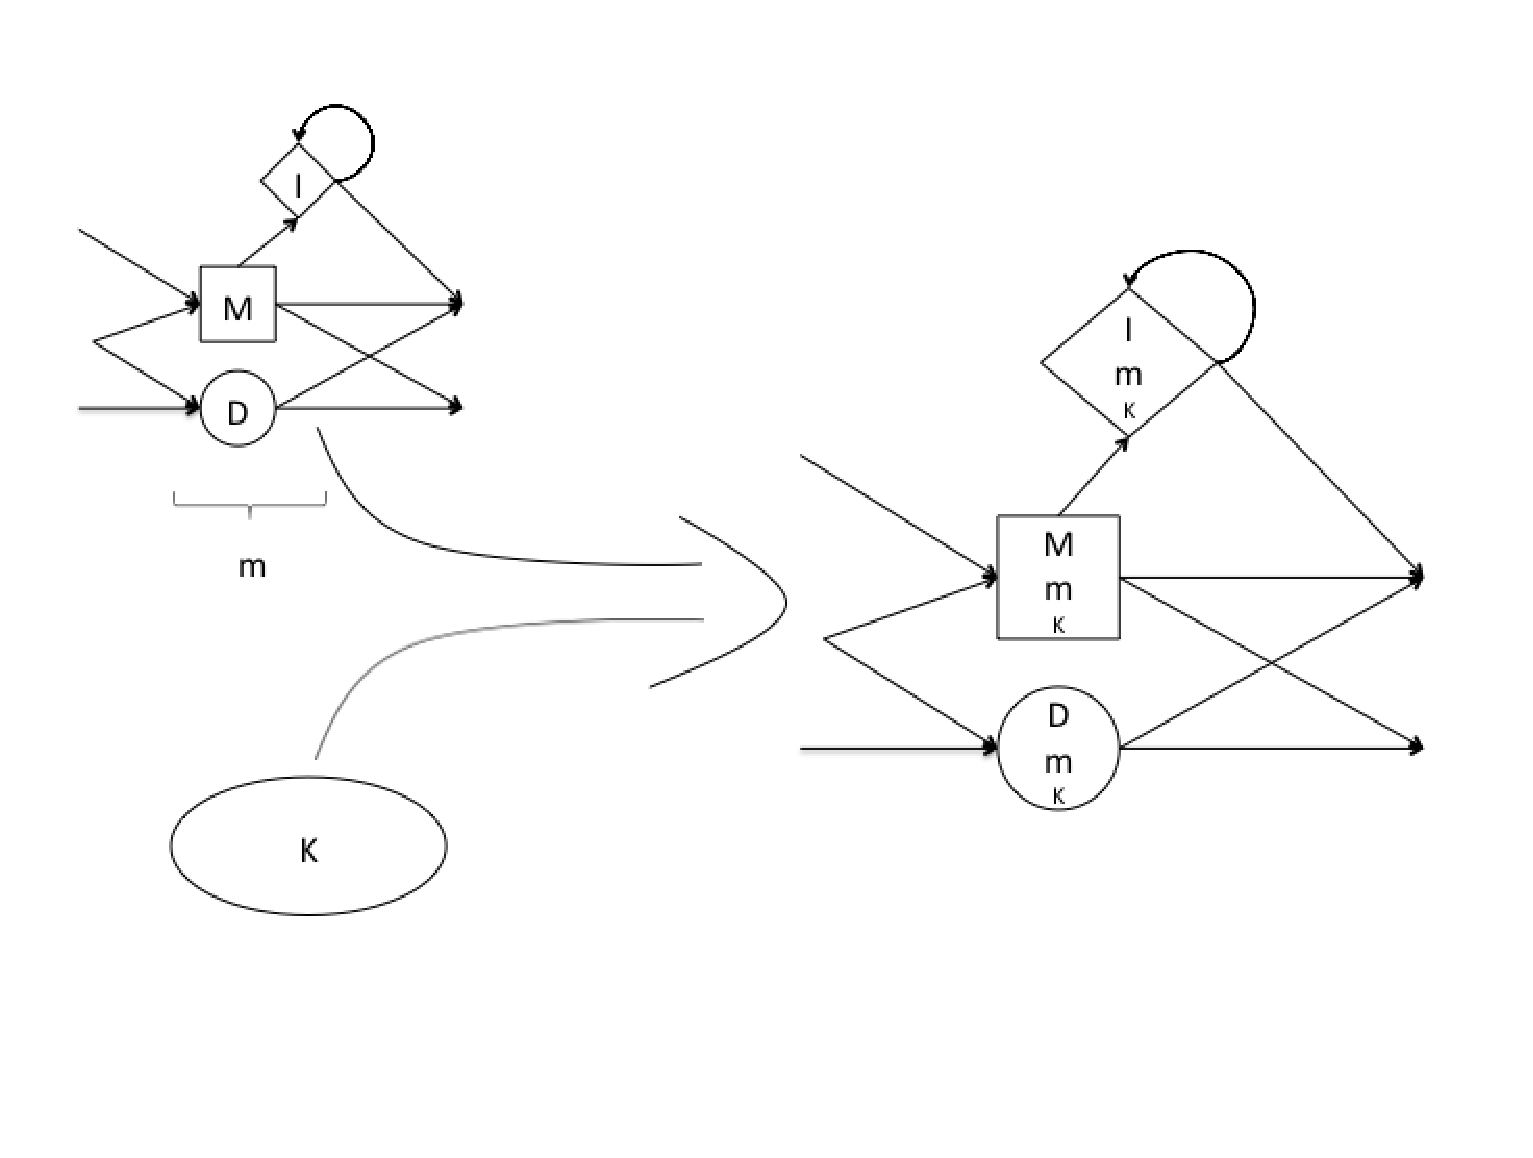
\includegraphics[width=117mm]{combined_graph.eps}
   \subsection*{Figure 2}
   	\includegraphics[width=120mm]{jaccard/paper_jaccard.eps}



%%%%%%%%%%%%%%%%%%%%%%%%%%%%%%%%%%%
%%                               %%
%% Tables                        %%
%%                               %%
%%%%%%%%%%%%%%%%%%%%%%%%%%%%%%%%%%%

%% Use of \listoftables is discouraged.
%%
\section*{Tables}
  \subsection*{Table 1 - Sample table title}
    Here is an example of a \emph{small} table in \LaTeX\ using  
    \verb|\tabular{...}|. This is where the description of the table 
    should go. \par \mbox{}
    \par
    \mbox{
		\begin{tabular}{| p{17mm} | p{15mm} | l | l | l | l |}
		\hline
		Dataset & Unique Starting vertices & Contigs Generated & Time (s) & Contigs merged & Unique\\
		\hline
		Iowa Corn & 2169 & 4035 & 2481 & 73 & 3 \\
		\hline
		Iowa Prairie & 3472 & 6671 & 3268 & 922 & 62 \\
		\hline
		Miscanthus Rizosphere & 23788 & 46493 & 15487 & 2379 & 262 \\
		\hline
	\end{tabular}
      }
  \subsection*{Table 2 - Sample table title}
    Large tables are attached as separate files but should
    still be described here.



%%%%%%%%%%%%%%%%%%%%%%%%%%%%%%%%%%%
%%                               %%
%% Additional Files              %%
%%                               %%
%%%%%%%%%%%%%%%%%%%%%%%%%%%%%%%%%%%

\section*{Additional Files}
  \subsection*{Additional file 1 --- Sample additional file title}
    Additional file descriptions text (including details of how to
    view the file, if it is in a non-standard format or the file extension).  This might
    refer to a multi-page table or a figure.

  \subsection*{Additional file 2 --- Sample additional file title}
    Additional file descriptions text.


\end{bmcformat}
\end{document}







